\chapter{Model Theory}\label{chapter:model-theory}

In this chapter, we will step away from the typical applications of logic in computer science\footnote{For example, using resolution to determine whether a given sentence $\varphi$ holds in a given finite theory $T$.} and look at a higher level of abstraction in the field of \emph{mathematical} logic. \emph{Model theory} seeks to describe the relationship between the general properties of theories (predicate logic) and the classes of their models. We will inevitably work with infinite theories and infinite structures. This is just a sample of some selected results that are accessible to us. We will not attempt to cover all the main areas of model theory, which is very rich and deep. We have also included material related to the properties of models in this chapter that did not fit elsewhere.

\section{Elementary Equivalence}

First, we will look at some properties related to the concept of \emph{elementary equivalence}. Recall that $L$-structures $\A$ and $\B$ are \emph{elementarily equivalent} ($\A\equiv \B$) if they satisfy the same $L$-sentences.

In model theory, we are often interested in what properties (sentences) hold in a given, specific structure:

\begin{definition}[Theory of a Structure]
Given an $L$-structure $\A$, the \emph{theory of the structure} $\A$, denoted $\Th(\A)$, is the set of all $L$-sentences that hold in $\A$:
$$
\Th(\A)=\{\varphi\mid\varphi \text{ is an $L$-sentence and } \A\models\varphi\}
$$
\end{definition}

\begin{example}
As an important example, consider the \emph{standard model of arithmetic}, the structure $\underline{\mathbb{N}}=\langle\mathbb{N},S,+,\cdot,0,\le\rangle$. The theory $\Th(\underline{\mathbb{N}})$ is called the \emph{arithmetic of natural numbers}. In the next chapter, we will show that it is \emph{(algorithmically) undecidable}.\footnote{A theory $T$ is \emph{(algorithmically) decidable} if there is an algorithm that, for every input sentence $\varphi$, terminates and answers whether $T\models\varphi$.}
\end{example}

We summarize several simple properties of the theory of a structure in the following observation:

\begin{observation}
    Let $\A$ be an $L$-structure and $T$ be an $L$-theory. Then:
    \begin{enumerate}[(i)]
        \item The theory $\Th(\A)$ is complete.
        \item If $\A\in\M_L(T)$, then $\Th(\A)$ is a (complete) simple extension of the theory $T$.
        \item If $\A\in\M_L(T)$ and $T$ is complete, then $\Th(\A)$ is equivalent to $T$, in which case $\Th(\A)=\Conseq_L(T)$.
    \end{enumerate}    
\end{observation}

Using the concept of the \emph{theory of a structure}, we can also express elementary equivalence. For $L$-structures $\A,\B$, it holds that:
$$
\A\equiv\B \text{ if and only if }\Th(\A)=\Th(\B).
$$

\begin{example}
   Consider the standard orderings of the reals, rationals, and integers, i.e., the structures $\langle\mathbb{R},\leq\rangle$, $\langle\mathbb{Q},\leq\rangle$, and $\langle\mathbb{Z},\leq\rangle$. As mentioned in Example \ref{example:elementary-equivalence-of-orders-R-Q}, it is not difficult to show that $\langle\mathbb{R},\leq\rangle\equiv\langle\mathbb{Q},\leq\rangle$ (using the \emph{density} of these orderings). However, the structures $\langle\mathbb{Q},\leq\rangle$ and $\langle\mathbb{Z},\leq\rangle$ are not elementarily equivalent: In $\langle\mathbb{Z},\leq\rangle$, every element has an immediate successor, which is not true in $\langle\mathbb{Q},\leq\rangle$. For the following sentence $\varphi$, we have $\varphi\in\Th(\langle\mathbb{Z},\leq\rangle)$ but $\varphi\not\in\Th(\langle\mathbb{Q},\leq\rangle)$:
   $$
   \varphi=(\forall x)(\exists y)(x\leq y \land \neg x=y \land (\forall z)(x\leq z \limplies z=x\lor y\leq z))
   $$
\end{example}

\subsection{Complete Simple Extensions}

Given a theory $T$, we are interested in what its models look like. Recall that:
\begin{itemize}
    \item A theory is \emph{complete} if it has a single model up to elementary equivalence.\footnote{That is, all its models are elementarily equivalent.}
    \item The models of a theory $T$ up to elementary equivalence correspond uniquely to the complete simple extensions of $T$.
\end{itemize}
The complete simple extensions of an $L$-theory $T$ are thus of the form $\Th(\A)$ for $\A\in\M_L(T)$, and (as mentioned above) $\A\equiv\B$ if and only if $\Th(\A)=\Th(\B)$. Instead of finding all models, it suffices to find all complete simple extensions.

\begin{remark}
    One motivation for dealing with complete simple extensions is Proposition \ref{propositon:recursively-enumerable-completion} from the next chapter, which states that if we can \emph{effectively (algorithmically) describe} all complete simple extensions\footnote{Imagine an algorithm that, for given inputs $i,j$, returns the $j$-th axiom of the $i$-th complete simple extension (in some fixed numbering); such an algorithm does not always exist!} of a \emph{given} theory $T$,\footnote{$T$ can be infinite, but there must be an algorithm that gradually generates all axioms of $T$.} then $T$ is \emph{(algorithmically) decidable}.
\end{remark}

The ability to (effectively) describe all complete simple extensions is relatively rare and requires strong assumptions. However, it can be done for many important theories. Let's give one example: the \emph{theory of dense linear orders (dense linear order)}.

\subsubsection{Example: DeLO*}

The theory of \emph{dense linear order (DeLO*)} is an extension of the theory of order by the following axioms:
\begin{itemize}
    \item the \emph{linearity} axiom (sometimes called the \emph{dichotomy} axiom):
    $$
    x \leq y \lor y \leq x
    $$
    \item the \emph{density} axiom:
    $$
    {x \leq y} \land {\neg x = y} \limplies (\exists z)(x \leq z \land z \leq y \land \neg z = x \land \neg z = y)
    $$
\end{itemize}
Sometimes, the \emph{non-triviality} axiom $(\exists x)(\exists y)(\neg x = y)$ is added to exclude the one-element model. This theory is not complete, but we can describe all its complete simple extensions:

\begin{proposition}
Let $\varphi = (\exists x)(\forall y)(x \leq y)$ and $\psi = (\exists x)(\forall y)(y \leq x)$ express the existence of a minimal or maximal element, respectively. The following four theories are exactly all (up to equivalence) complete simple extensions of the DeLO* theory:
\begin{itemize}
    \item $\DeLO = \DeLO^* \ \cup \ \{\neg\varphi, \neg\psi\}$
    \item $\DeLO^+ = \DeLO^* \ \cup \ \{\neg\varphi, \psi\}$
    \item $\DeLO^- = \DeLO^* \ \cup \ \{\varphi, \neg\psi\}$
    \item $\DeLO^\pm = \DeLO^* \ \cup \ \{\varphi, \psi\}$        
\end{itemize}
\end{proposition}

It suffices to show that these four theories are complete. Then it is clear that no other complete simple extension of DeLO* can exist. As we will explain in Section \ref{section:categoricity}, their completeness follows from the fact that they are \emph{$\omega$-categorical}, i.e., they have a unique countable model up to \emph{isomorphism}. See Corollary \ref{corollary:complete-simple-extensions-of-delo}.

\subsection{Consequences of Löwenheim-Skolem Theorem}

In Section \ref{subsection:loewenheim-skolem-theorem}, we proved the Löwenheim-Skolem theorem, specifically its variant for languages without equality:

\begin{theorem-unnumbered}[Löwenheim-Skolem]
    If $L$ is a countable language without equality, then every consistent $L$-theory has a countably infinite model.
\end{theorem-unnumbered}

This theorem has the following simple corollary:

\begin{corollary}\label{corollary:loewenheim-skolem-without-equality}
    If $L$ is a countable language without equality, then for every $L$-structure, there exists an elementarily equivalent countably infinite structure.
\end{corollary}
\begin{proof}
    Given an $L$-structure $\A$. The theory $\Th(\A)$ is consistent (it has a model $\A$), so by the Löwenheim-Skolem theorem, it has a countably infinite model $\B\models\Th(\A)$. This means that $\B\equiv\A$.
\end{proof}

In a language without equality, we cannot express, for example, that `the model has exactly 42 elements'.

In the proof of the Löwenheim-Skolem theorem, we obtained the constructed model as the canonical model for the consistent branch of the tableau from $T$ for the entry $\F\bot$. The following version for languages with equality is proved in the same way, just by factoring through the relation $=^A$:

\begin{theorem-unnumbered}[Löwenheim-Skolem with Equality]
    If $L$ is a countable language with equality, then every consistent $L$-theory has a countable model (i.e., finite or countably infinite).
\end{theorem-unnumbered}

This version also has an easy corollary for specific structures:

\begin{corollary}\label{corollary:loewenheim-skolem-with-equality}
    If $L$ is a countable language with equality, then for every \emph{infinite} $L$-structure, there exists an elementarily equivalent countably infinite structure.
\end{corollary}
\begin{proof}
    Given an infinite $L$-structure $\A$. As in the proof of Corollary \ref{corollary:loewenheim-skolem-without-equality} (but using the Löwenheim-Skolem theorem with equality), we find a countable structure $\B\equiv\A$. Since in $\A$ every $n\in\mathbb{N}$ satisfies sentences expressing `there exist at least $n$ elements' (which can be easily written using equality), these sentences hold in $\B$ as well, so $\B$ cannot be finite and must be countably infinite.
\end{proof}

We will use this corollary to show that there exists a countable field that is algebraically closed:

\subsubsection*{Countable Algebraically Closed Field}

A field $\A$ is \emph{algebraically closed} if every non-zero degree polynomial has a root in it. The field of real numbers $\mathbb{R}$ is not algebraically closed because $x^2+1$ has no root in $\mathbb{R}$, and similarly, the field of rationals $\mathbb{Q}$ is not (as $x^2-2$ has no root in $\mathbb{Q}$). The field of complex numbers $\mathbb{C}$ is algebraically closed, but it is uncountable.

Algebraic closure can be expressed using the following sentences $\psi_n$, for each $n>0$:
$$
(\forall x_{n-1})\dots(\forall x_0)(\exists y)(y^n+x_{n-1}\cdot y^{n-1}+\dots+x_1\cdot y + x_0) = 0
$$
where $y^k$ is shorthand for the term $y \cdot y \cdot \cdots \cdot y$ (where $\cdot$ is applied $(k-1)$ times).

\begin{corollary}
    There exists a countable algebraically closed field.
\end{corollary}
\begin{proof}
    By Corollary \ref{corollary:loewenheim-skolem-with-equality}, there exists a countably infinite structure $\A$ elementarily equivalent to the field $\mathbb{C}$. Since $\mathbb{C}$ is a field and satisfies the sentences $\psi_n$ for all $n>0$, $\A$ is also an algebraically closed field.
\end{proof}

\section{Isomorphism of Structures}\label{section:isomorphism-of-structures}

Let's take a closer look at the concept of \emph{isomorphism of structures}, which generalizes the isomorphism of graphs, vector spaces, etc. Informally, structures are \emph{isomorphic} if they differ only in the naming of specific elements.

\begin{definition}
Given structures $\A, \B$ in a language $L = \langle\mathcal{R}, \mathcal{F}\rangle$, an \emph{isomorphism between $\A$ and $\B$} (or `from $\A$ to $\B$') is a bijection $h\colon A \to B$ satisfying the following properties:
\begin{itemize}
    \item For each ($n$-ary) function symbol $f \in \mathcal{F}$ and for all $a_i \in A$, it holds that:
    $$
    h(f^\A(a_1, \dots, a_n)) = f^\B(h(a_1), \dots, h(a_n))
    $$
    (Specifically, if $c \in \mathcal{F}$ is a constant symbol, it holds that $h(c^\A) = c^\B$.)
    \item For each ($n$-ary) relation symbol $R \in \mathcal{R}$ and for all $a_i \in A$, it holds that:
    $$
    R^\A(a_1, \dots, a_n)\ \text{ if and only if }\ R^\B(h(a_1), \dots, h(a_n))
    $$
\end{itemize}
If an isomorphism exists, we say that $\A$ and $\B$ are \emph{isomorphic} (or `$\A$ is \emph{isomorphic to $\B$ via $h$}') and write $\A \simeq \B$ (or $\A \simeq_h \B$). An \emph{automorphism} of $\A$ is an isomorphism from $\A$ to $\A$.
\end{definition}

Note that the relation `being isomorphic' is an equivalence relation. Let's look at an example:

\begin{example}
    If $|X| = n$, the power set algebra $\underline{\mathcal{P}(X)} = \langle \mathcal{P}(X), -, \cap, \cup, \emptyset, X\rangle$ is isomorphic to the Boolean algebra $\underline{2^n} = \langle \{0,1\}^n, -_n, \land_n, \lor_n, (0, \dots, 0), (1, \dots, 1)\rangle$ (where the operations are applied component-wise) via $h(A) = \chi_A$, where $\chi_A$ is the characteristic vector of the subset $A \subseteq X$.
\end{example}

Now we show that an isomorphism is a bijection that `preserves semantics':

\begin{proposition}
Given structures $\A, \B$ in a language $L = \langle\mathcal{R}, \mathcal{F}\rangle$. A bijection $h\colon A \to B$ is an isomorphism between $\A$ and $\B$ if and only if the following hold:
\begin{enumerate}[(i)]
    \item For every $L$-term $t$ and variable assignment $e\colon \Var \to A$:
    $$
    h(t^\A[e]) = t^\B[e \circ h]
    $$
    \item For every $L$-formula $\varphi$ and variable assignment $e\colon \Var \to A$:
    $$
    \A \models \varphi[e]\ \text{ if and only if }\ \B \models \varphi[e \circ h]
    $$
\end{enumerate}
\end{proposition}
\begin{proof}
    If $h$ is an isomorphism, the properties are easily proved by induction on the structure of the term or formula. Conversely, if $h$ is a bijection satisfying (i) and (ii), substituting $t = f(x_1, \dots, x_n)$ and $\varphi = R(x_1, \dots, x_n)$ gives the properties from the definition of isomorphism.
\end{proof}

As an immediate consequence, we get the fact that isomorphic structures are elementarily equivalent:

\begin{corollary}\label{corollary:isomorphic-implies-elementarily-equivalent}
    If $\A \simeq \B$, then $\A \equiv \B$.
\end{corollary}

\begin{remark}
    The converse implication does not generally hold. For example, for ordered sets of rational and real numbers, $\langle\mathbb{Q}, \leq \rangle \equiv \langle\mathbb{R}, \leq \rangle$, but $\langle\mathbb{Q}, \leq \rangle \not\simeq \langle \mathbb{R}, \leq \rangle$ because $\mathbb{Q}$ is a countable set while $\mathbb{R}$ is not (so there is no bijection between them).
\end{remark}

For finite models, however, isomorphism is the same as elementary equivalence if we have a language with equality, as we will prove in the following proposition:

\begin{proposition}
    If $L$ is a language with equality and $\A, \B$ are finite $L$-structures, then:
    $$
    \A \simeq \B\ \text{ if and only if }\ \A \equiv \B
    $$
\end{proposition}
\begin{proof}
    We proved one implication in Corollary \ref{corollary:isomorphic-implies-elementarily-equivalent}. Suppose $\A \equiv \B$ and show that there is an isomorphism from $\A$ to $\B$. Since the language includes equality, we can express by a sentence that `there are exactly $n$ elements'. This implies that $|A| = |B|$.

    Let $\A'$ be the expansion of $\A$ by names of elements from $A$; it is a structure in the language $L' = L \cup \{c_a \mid a \in A\}$. We will show that $\B$ can be expanded to an $L'$-structure $\B$ such that $\A' \equiv \B'$. Then, as can be easily verified, the mapping $h(a) = c_a^{\B'}$ is an isomorphism from $\A'$ to $\B'$, and thus also an isomorphism of their $L$-reducts and $\A \simeq \B$.

    It suffices to show that for each $c_a^{\A'} = a \in A$, there exists an element $b \in B$ such that for expansions with the interpretation of the constant symbol $c_a$, it holds that $\langle \A, a \rangle \equiv \langle \B, b \rangle$. Let $\Omega$ be the set of formulas $\varphi(x)$ such that $\langle \A, a \rangle \models \varphi(x/c_a)$, i.e., $\A \models \varphi[e(x/a)]$. Since $A$ is a finite set, there are finitely many formulas $\varphi_1(x), \dots, \varphi_m(x)$ such that for each formula $\varphi \in \Omega$, there exists $i$ such that $\A \models \varphi \liff \varphi_i$. Then $\B \models \varphi \liff \varphi_i$ (since $\A \equiv \B$, just take the general closure of this formula, which is a sentence).
    
    Since in $\A$ the sentence $(\exists x)\bigwedge_{i=1}^m \varphi_i$ holds (it is satisfied by the element $a \in A$), and $\B \equiv \A$, we also have $\B \models (\exists x)\bigwedge_{i=1}^m \varphi_i$. In other words, there exists $b \in B$ such that $\B \models \bigwedge_{i=1}^m \varphi_i[e(x/b)]$. Thus, for each $\varphi \in \Omega$, $\B \models \varphi[e(x/b)]$, i.e., $\langle \mathcal{B}, b \rangle \models \varphi(x/c_a)$, which is what we wanted to prove.
\end{proof}

\begin{corollary}
    If a complete theory in a language with equality has a finite model, then all its models are isomorphic.
\end{corollary}

\subsection{Definability and Automorphisms}

Recall the concept of a definable set from Section \ref{section:definability}. We will show a useful property of definable sets: they are closed (`invariant') under automorphisms of the given structure.

It should surprise no one that under an automorphism, an isolated vertex of a given graph must map to an isolated vertex, a vertex of degree 4 to a vertex of the same degree, or a triplet of vertices forming a triangle to a triangle. This can help us, for example, in finding automorphisms.

\begin{proposition}
    If $D \subseteq A^n$ is definable in the structure $\A$, then for every automorphism $h \in \Aut(\A)$, it holds that $h[D] = D$ (where $h[D]$ denotes $\{h(\overline{a}) \mid \overline{a} \in D\}$).

    If $D$ is definable with parameters $\overline{b}$, the same holds for automorphisms that are identical on $\overline{b}$, i.e., such that $h(\overline{b}) = \overline{b}$ (meaning $h(b_i) = b_i$ for all $i$).
\end{proposition}
\begin{proof}
    We will show only the version with parameters. Let $D = \varphi^{\A, \overline{b}}(\overline{x}, \overline{y})$. Then for every $\overline{a} \in A^n$, the following equivalence holds:
\begin{align*}
\overline{a} \in D\ 
&\Leftrightarrow\ \A \models \varphi[e(\overline{x}/\overline{a}, \overline{y}/\overline{b})] \\
&\Leftrightarrow\ \A \models \varphi[(e \circ h)(\overline{x}/\overline{a}, \overline{y}/\overline{b})] \\
&\Leftrightarrow\ \A \models \varphi[e(\overline{x}/h(\overline{a}), \overline{y}/h(\overline{b}))] \\
&\Leftrightarrow\ \A \models \varphi[e(\overline{x}/h(\overline{a}), \overline{y}/\overline{b})] \\
&\Leftrightarrow\ h(\overline{a}) \in D.
\end{align*}
\end{proof}

\begin{example}
    Consider the following graph $\mathcal{G}$. Find all sets definable from $\mathcal{G}$ with parameter $0$, i.e., the set $\mathrm{Df}^1(\mathcal{G}, \{0\})$. 
    \begin{center}
        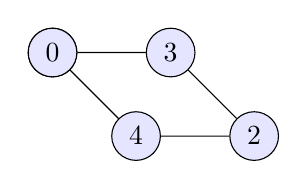
\begin{tikzpicture}[every node/.style={circle,fill=blue!10,draw,minimum size=0.5cm,node distance=1.5cm}]
        \node (1) {$1$};
        \node (0) {$0$};
        \node[below right of=0] (4) {$4$};
        \node[right of=4] (3) {$2$};
        \node[right of=1] (2) {$3$};
        \path[draw] (0) -- (1) -- (2) -- (3) -- (4) -- (0);
        \end{tikzpicture}
        \end{center}
    This graph has a single non-trivial automorphism preserving the vertex $0$: $h(i) = (5 - i) \bmod 5$. Its \emph{orbits} are $\{0\}$, $\{1, 4\}$, and $\{2, 3\}$. These sets are definable:
    \begin{itemize}
        \item $\{0\}$ is defined by the formula $x = y$, i.e., $(x = y)^{\mathcal{G}, \{0\}} = \{0\}$,
        \item $\{1, 4\}$ can be defined by the formula $E(x, y)$, and
        \item $\{2, 3\}$ by the formula $\neg E(x, y) \land \neg x = y$.
    \end{itemize}
    The set $\mathrm{Df}^1(\mathcal{G}, \{0\})$ is a subalgebra of the power set algebra $\underline{\mathcal{P}(V(\mathcal{G}))}$, so it must be closed under complement, union, intersection, and contain $\emptyset$ and $V(\mathcal{G})$. The subalgebra generated by $\{\{0\}, \{1, 4\}, \{2, 3\}\}$, however, contains all the subsets preserving the automorphism $h$. We get:
    $$
    \mathrm{Df}^1(\mathcal{G}, \{0\}) = \{\emptyset, \{0\}, \{1, 4\}, \{2, 3\}, \{0, 1, 4\}, \{0, 2, 3\}, \{1, 2, 3, 4\}, \{0, 1, 2, 3, 4\}\}
    $$
\end{example}

\begin{exercise}
    Consider the following graph. Find all automorphisms. Determine which subsets are definable, provide defining formulas. Which binary relations are definable?
    \begin{center}
        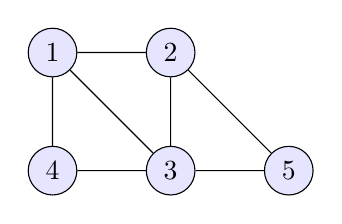
\begin{tikzpicture}[every node/.style={circle,fill=blue!10,draw,minimum size=0.5cm,node distance=1.5cm}]
            \node (1) {$1$};
            \node[right of=1] (2) {$2$};
            \node[below of=2] (3) {$3$};
            \node[left of=3] (4) {$4$};
            \path[draw] (1) -- (2) -- (3) -- (4) -- (1) -- (3);
            \node[right of=3] (5) {$5$};
            \path[draw] (2) -- (5) -- (3);
        \end{tikzpicture}
    \end{center}
\end{exercise}


\section{$\omega$-categorical Theories}\label{section:categoricity}

Now we will look at theories that have a single countably infinite model (up to isomorphism); these are called \emph{$\omega$-categorical} theories.\footnote{The symbol $\omega$ is used for the smallest infinite \emph{ordinal} number, in other words, the set of all natural numbers.}

\begin{definition}[Isomorphism Spectrum, $\kappa$-categoricity]
    The \emph{isomorphism spectrum} of a theory $T$ is the number $
    I(\kappa,T)$ of models of $T$ of cardinality $\kappa$ up to isomorphism, for each cardinality $\kappa$ (including \emph{transfinite} ones). A theory $T$ is \emph{$\kappa$-categorical} if $
    I(\kappa,T)=1$.
\end{definition}

From now on, we will be interested only in the case $\kappa=\omega$, that is, theories with a single countably infinite model (up to isomorphism). As an example, consider the theory of dense linear orderings without endpoints:

\begin{proposition}
    The theory DeLO is $\omega$-categorical.
\end{proposition}
\begin{proof}
Consider two countably infinite models $\A, \B$, and enumerate their elements: $A=\{a_i \mid i\in \mathbb{N}\}$, $B=\{b_i \mid i\in \mathbb{N}\}$. By induction on $n$, we can, thanks to density, find a sequence $h_0 \subseteq h_1 \subseteq h_2 \subseteq \dots$ of injective (partial) functions from $A$ to $B$ such that $\{a_0, \dots, a_{n-1}\} \subseteq \dom h_n$, $\{b_0, \dots, b_{n-1}\} \subseteq \rng h_n$,\footnote{Here, $\dom$ denotes the \emph{domain} and $\rng$ denotes the \emph{range} of a function.} and \emph{preserve the order}\footnote{That is, if $a_i, a_j \in \dom h_n$, then $a_i \leq^\A a_j$ if and only if $h(a_i) \leq^\B h(a_j)$.} Then $\A \simeq \B$ via $h = \bigcup_{n\in \mathbb{N}} h_n$.
\end{proof}

\begin{corollary}
The isomorphism spectrum of the theory DeLO* is as follows:
$$
I(\kappa, DeLO^*)=\begin{cases}
    0 &\text{for } \kappa \in \mathbb{N},\\
    4 &\text{for } \kappa = \omega.
\end{cases}
$$
Countable models up to isomorphism are, for example:
$$ 
\mathbb{Q} = \langle \mathbb{Q}, \leq \rangle \simeq \mathbb{Q} \upharpoonright (0,1), \ \mathbb{Q} \upharpoonright (0,1], \ \mathbb{Q} \upharpoonright [0,1), \ \mathbb{Q} \upharpoonright [0,1]
$$
\end{corollary}

\begin{proof}
A dense order cannot be finite. An isomorphism must map the smallest element to the smallest element and the largest to the largest.
\end{proof}

The concept of \emph{$\omega$-categoricity} can be understood as a weakening of the concept of \emph{completeness}. The following useful criterion applies:

\begin{theorem}[$\omega$-Categorical Completeness Criterion]
Let $T$ be an $\omega$-categorical theory in a countable language $L$. If
\begin{itemize}
    \item $L$ is without equality, or
    \item $L$ is with equality and $T$ has no finite models,
\end{itemize}
then the theory $T$ is complete.
\end{theorem}
\begin{proof}
For a language without equality, we know from Corollary \ref{corollary:loewenheim-skolem-without-equality} of the Löwenheim-Skolem theorem that every model is elementarily equivalent to some countably infinite model. However, that model is unique up to isomorphism, so all models are elementarily equivalent, which is the semantic definition of completeness.

For a language with equality, we similarly use Corollary \ref{corollary:loewenheim-skolem-with-equality} and obtain that all infinite models are elementarily equivalent. There could exist elementarily nonequivalent finite models, but we have excluded that possibility.
\end{proof}

\begin{corollary}\label{corollary:complete-simple-extensions-of-delo}
    The theories $\DeLO$, $\DeLO^+$, $\DeLO^-$, and $\DeLO^\pm$ are complete. These are all (mutually nonequivalent) complete simple extensions of the theory $DeLO^*$.
\end{corollary}

\begin{remark}
An analogous criterion applies for cardinalities $\kappa$ greater than $\omega$.
\end{remark}

\section{Axiomatizability}\label{section:axiomatizability}

Finally, in this chapter, we will look at the circumstances under which a class of models or a theory can be `described' (\emph{axiomatized}). We will also be interested in when we can manage with finitely many axioms and when it can be done with open axioms (which may be infinitely many). Compare with Proposition \ref{proposition:axiomatize-in-DNF-CNF} from propositional logic.

\begin{definition}[Axiomatizability]
Let $K \subseteq \M_L$ be a class of structures in some language $L$. We say that $K$ is
\begin{itemize}
    \item \emph{axiomatizable} if there exists an $L$-theory $T$ such that $\M_L(T)=K$,
    \item \emph{finitely axiomatizable} if it is axiomatizable by a finite theory, and
    \item \emph{openly axiomatizable} if it is axiomatizable by an open theory.
\end{itemize}
We say that an $L$-theory $T'$ is \emph{finitely} or \emph{openly axiomatizable} if this applies to the class of models $K=\M_L(T')$.
\end{definition}

\begin{example}
    Here are some examples:
    \begin{itemize}
        \item Graphs or partial orders are both finitely and openly axiomatizable.
        \item Fields are finitely but not openly axiomatizable.
        \item Infinite groups are axiomatizable but not finitely.
        \item Finite graphs are not axiomatizable.
    \end{itemize}
    We will explain why this is so below.
\end{example}

Let's start with a simple fact:

\begin{observation}
    If $K$ is axiomatizable, it must be closed under elementary equivalence.  
\end{observation}

From the compactness theorem, we easily obtain the following statement, which can be used to show the non-axiomatizability of, for example, finite graphs, finite groups, and finite fields.

\begin{theorem}
    If a theory has arbitrarily large finite models, then it also has an infinite model. In that case, the class of all its finite models is not axiomatizable.
\end{theorem}
\begin{proof}
    If the language is without equality, it suffices to take the canonical model for some consistent branch in the tableau from $T$ for the entry $\F\bot$ ($T$ is consistent, as it has models, so the tableau is not inconsistent).     
    
    Suppose we have a language with equality, and let $T'$ be the following extension of the theory $T$ to the language expanded by countably many new constant symbols $c_i$:
    $$
    T'=T \cup \{\neg c_i = c_j \mid i \neq j \in \mathbb{N}\}
    $$
    Every finite part of the theory $T'$ has a model: let $k$ be the largest such that the symbol $c_k$ appears in this finite part of $T'$. Then it suffices to take any model of $T$ with at least $(k+1)$ elements and interpret the constants $c_0, \dots, c_k$ as distinct elements of this model.

    By the compactness theorem, $T'$ also has a model. That model is necessarily infinite. Its reduct to the original language (forgetting the constants $c_i^\A$) is an infinite model of $T$.
\end{proof}

\begin{remark}
    The class of all \emph{infinite} models of a theory is always axiomatizable if we have a language with equality: it suffices to add to the theory, for each $n \in \mathbb{N}$, an axiom expressing `there are at least $n$ elements'.
\end{remark}

\subsection{Finite Axiomatizability}

We will show the following criterion for finite axiomatizability: both the class of structures $K$ and its complement $\overline{K}$ must be axiomatizable.

\begin{theorem}[Finite Axiomatizability]\label{theorem:finite-axiomatizability}
    Let $K \subseteq \M_L$ be a class of structures and also consider its complement $\overline{K} = \M_L \setminus K$. Then $K$ is finitely axiomatizable if and only if both $K$ and $\overline{K}$ are axiomatizable.   
\end{theorem}
\begin{proof}
If $K$ is finitely axiomatizable, then it is axiomatizable by finitely many sentences $\varphi_1, \dots, \varphi_n$ (we replace formulas with their general closures). To axiomatize $\overline{K}$, it suffices to take the sentence $\psi = \neg(\varphi_1 \land \varphi_2 \land \dots \land \varphi_n)$. Clearly, $\M(\psi) = \overline{K}$.

Conversely, suppose $T$ and $S$ are theories such that $\M(T) = K$ and $\M(S) = \overline{K}$. Consider the theory $T \cup S$. This theory is inconsistent, as:
$$
\M(T \cup S) = \M(T) \cap \M(S) = K \cap \overline{K} = \emptyset
$$
By the compactness theorem,\footnote{You can see how useful it is!} there exist finite subtheories $T' \subseteq T$ and $S' \subseteq S$ such that:
$$
\emptyset = \M(T' \cup S') = \M(T') \cap \M(S')
$$
Now note that:
$$
\M(T) \subseteq \M(T') \subseteq \overline{\M(S')} \subseteq \overline{\M(S)} = \M(T)
$$
Thus, we have shown that $\M(T) = \M(T')$, that is, the theory $T'$ is the desired finite axiomatization of $K$.
\end{proof}

As an application, we will prove that fields of characteristic 0 are not finitely axiomatizable.

\subsubsection*{Example: Fields of Characteristic 0}
 
Let $T$ be the theory of fields. The characteristic of a field is the smallest number of ones that must be added to get zero (in that case, the characteristic must be a prime number---prove it!), or if we never get zero by adding ones, we say that the characteristic is 0. More formally:

\begin{definition}[Characteristic of a Field]
We say that a field $\A = \langle A, +, -, 0, \cdot, 1 \rangle$ is of
\begin{itemize}
    \item \emph{characteristic $p$} if $p$ is the smallest prime number such that $\A \models p1 = 0$, where $p1$ denotes the term $1 + 1 + \dots + 1$ with $p$ ones, or
    \item \emph{characteristic 0} if it is not of characteristic $p$ for any prime number $p$.
\end{itemize}
\end{definition}
Let $T$ be the theory of fields. Then the class of fields of characteristic $p$ is finitely axiomatized by the theory $T \cup \{p1 = 0\}$. The class of fields of characteristic 0 is axiomatized by the following (infinite) theory:
$$
T' = T \cup \{\neg\, p1 = 0 \mid p \text{ is a prime number}\}
$$
However, a finite axiomatization does not exist.

\begin{proposition}
The class $K$ of fields of characteristic $0$ is not finitely axiomatizable.   
\end{proposition}
\begin{proof}
Thanks to Theorem \ref{theorem:finite-axiomatizability}, it suffices to show that $\overline{K}$ (consisting of fields of non-zero characteristic and structures that are not fields) is not axiomatizable, which we will prove by contradiction. Suppose there exists a theory $S$ such that $\M(S) = \overline{K}$. Then the theory 
$S' = S \cup T'$ has a model, as every finite part of it has a model: it suffices to take a field of prime characteristic greater than any $p$ from the axioms of $T'$ of the form $\neg\, p1 = 0$. Let $\A$ be a model of $S'$. Then $\A \in \M(S) = \overline{K}$. At the same time, $\A \in \M(T') = K$, which is a contradiction.
\end{proof}

\subsection{Open Axiomatizability}

For open axiomatizability, there is a simple semantic criterion: the class of its models must be closed under substructures. There is even an equivalence, but we will prove only one implication (the proof of the other is more difficult).

\begin{theorem}\label{theorem:open-axiomatizability}
If a theory $T$ is openly axiomatizable, then every substructure of a model of $T$ is also a model of $T$.   
\end{theorem}

\begin{remark}
    The converse implication also holds: If every substructure of a model of $T$ is also a model, then $T$ is openly axiomatizable. We will not provide the proof here.
\end{remark}

\begin{proof}
Suppose $T'$ is an open axiomatization of $T$. Let $\A \models T'$ be a model and $\B \subseteq \A$ be a substructure. For every formula $\varphi \in T'$, it holds that $\B \models \varphi$ (since $\varphi$ is open), thus $\B \models T'$.  
\end{proof}

\begin{example}
    Here are some examples:
    \begin{itemize}
        \item The theory DeLO is not openly axiomatizable; for example, no finite substructure of a model of DeLO can be dense.
        \item The theory of fields is not openly axiomatizable; the substructure $\mathbb{Z} \subseteq \mathbb{Q}$ of the field of rational numbers is not a field, as there is no multiplicative inverse of $2$ in $\mathbb{Z}$.
        \item For a given $n \in \mathbb{N}$, the theories of at most $n$-element groups are openly axiomatizable (subgroups are certainly also at most $n$-element). As an open axiomatization, we can take the following extension of the (open) theory of groups $T$:
        $$
        T \cup \{\bigvee_{1 \leq i < j \leq n+1} x_i = x_j\}
        $$
    \end{itemize}
\end{example}
